%% 内容梗概

%% プリアンブル %%%%%%%%%%%%%%%%%%%%%%%%%%%%%%%%%%%%%%%%%%%%%%%%%%%%%%%%
\documentclass[a4j]{jarticle}

\usepackage{kut-abstract}
\usepackage[dvips]{graphicx}
\usepackage{url}
\usepackage{here}
%% 表題 %%%%%%%%%%%%%%%%%%%%%%%%%%%%%%%%%%%%%%%%%%%%%%%%%%%%%%%%%%%%%%%%
%% 注意! 情報学群生の場合は,以下の \ScInfo を有効にすること.
\ScInfo        %% 情報学群生の場合

\Bachelor	%% 卒業研究論文梗概の場合
%\Project	%% プロジェクト研究報告書梗概の場合
%\Seminar	%% 特別研究セミナー課題研究報告書梗概の場合
%\Master	%% 修士学位論文(情報システム工学コース)梗概の場合
%\Doctorate	%% 博士学位論文(情報システム工学コース)梗概の場合
%\English	%% 英語の場合

\Eyears{2016}
\Etitle{English Title}
%\idnumber{}
\Eauthor{KAWAGUCHI, Takahiro}
\Eaffiliate{Yokoyama Lab.}

%% 本文 %%%%%%%%%%%%%%%%%%%%%%%%%%%%%%%%%%%%%%%%%%%%%%%%%%%%%%%%%%%%%%%%

\years{平成27}
\title{OpenStack環境でのオーケストレーション定義を容易にするGUIエディタの実現}
\idnumber{1160304}
\author{川口 ~~貴大}
\affiliate{横山研究室}

%% 本文 %%%%%%%%%%%%%%%%%%%%%%%%%%%%%%%%%%%%%%%%%%%%%%%%%%%%%%%%%%%%%%%%
\begin{document}
\begin{Abstract}
 
 \section{はじめに}
 近年,ITリソースの迅速な確保,コスト削減等の目的からシステムの基盤としてIaaSの需要が高まっている.代表的なIaaS基盤ソフトウェアとしてOpenStackが挙げられる.\cite{Document:1}システム設計では冗長化や負荷分散,処理の効率化といった理由により,複数マシンの構成となる場合が多く見られる.しかし,システムの流用や再利用が求められる場面では、大規模なシステムになるにつれ、マシン台数も増加し設定に掛かる工程が増大してしまう。そのため,システム再現における作業の効率化が求められている.
 
 \texttt OpenStackではHeatと呼ばれるオーケストレーション(自動構築)機能を提供するコンポーネントにより,システムの再現を効率化している.HeatではITリソースの構成情報を記述した設計図(テンプレートファイル)を読み込ませることで,その構成情報を基に自動的にシステムの構築を行う.しかし,テンプレートファイルは書式が複雑であり,記述を行う際にはHeat独自の知識を要する.またテキストファイルであるため,記述量の増加による構築ミス,作成所要時間の増大,構成情報がテキストからイメージし難いという問題も抱えている.
 
 \texttt 本研究ではGUIを用いたオーケストレーション定義エディタを提案し、従来方式の問題点を解決しつつ短時間かつ容易に仮想環境を構築できることを示した.
 \section{オーケストレーション定義エディタの提案と実装}
 \subsection{オーケストレーション定義エディタの概要}
 オーケストレーション定義エディタでは,構築中のシステム構成を可視化するためにGUIを採用している.オーケストレーション定義エディタの概略図を図\ref{graf:1}に示す.
 \begin{figure}[H]
 	\begin{center}
 		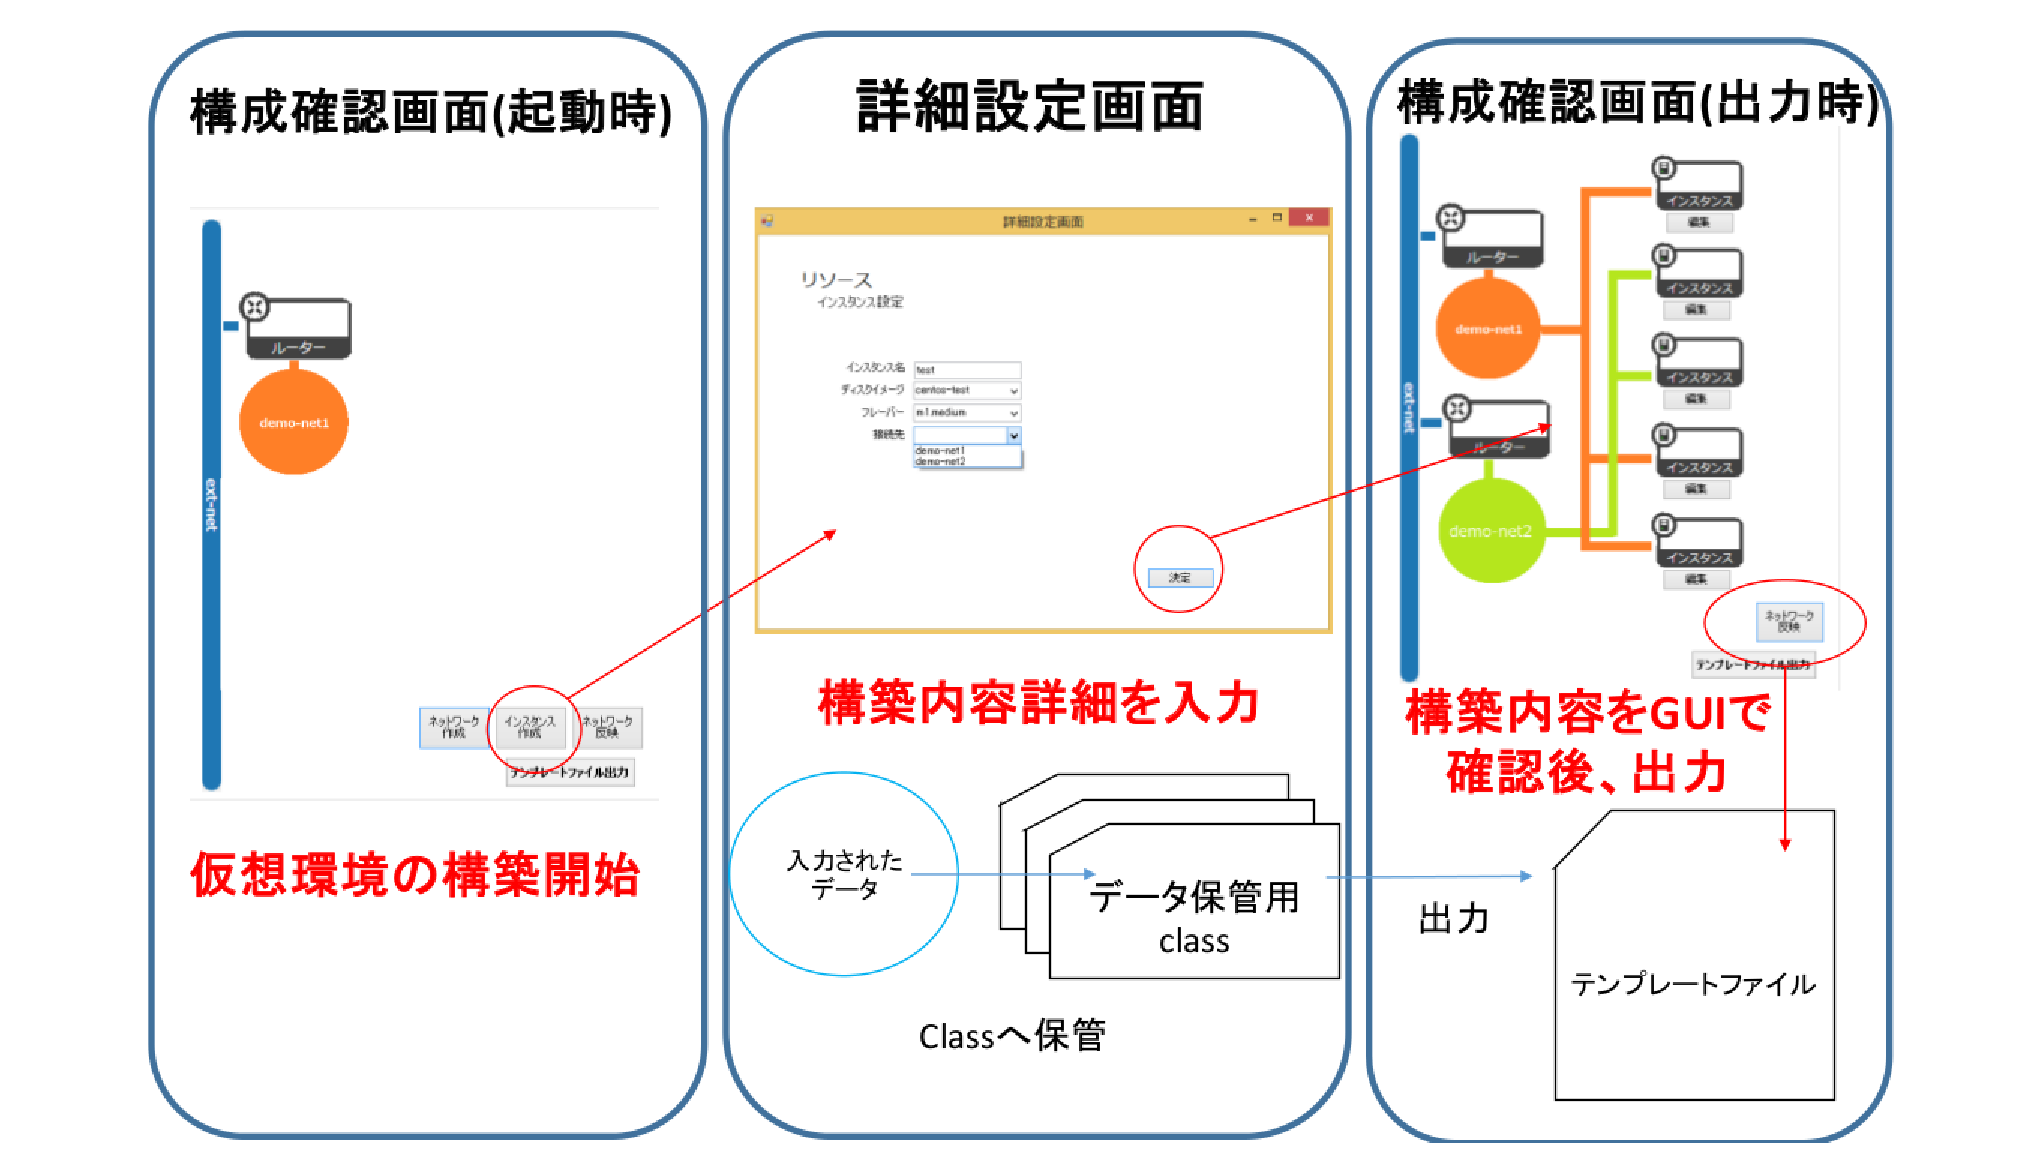
\includegraphics[scale=0.245]{Document/GUIEditorOverview.eps}
 		\caption{オーケストレーション定義エディタの概略}
 		\label{graf:1}
 	\end{center}
 \end{figure}
 \subsection{一部を除く手動入力項目の撤廃}
 オーケストレーション定義エディタでは従来方式の問題点のひとつであるテンプレートファイル作成時記述量の増加によるミスの改善,それに伴うテンプレートファイル作成所要時間を削減するために,インスタンス名入力項目以外の項目全てで手動入力方式を廃止,代わりにプルダウンメニューを採用した.これにより入力時間の大幅短縮,入力項目のエラー発生抑制を実現した.
% \begin{figure}[hbtp]
%  \begin{center}
%   \includegraphics[width=\columnwidth,clip]{im_outline}
%   \vspace{-2zh}
%   \caption{電子部品自動挿入機の概観}
%   \label{fig:im_outline}
%  \end{center}
% \end{figure}
% \vspace{-1zh}
% \begin{equation}
%  losstime = \sum_{i = 1}^{n - 1}l_{p(i) p(i + 1)} + l_{p(n) p(1)}
%   \label{eq:losstime}
% \end{equation}

 \section{評価}
 事前にOpenStackとHeat,オーケストレーション定義エディタについて学習した被験者5人に,従来方式とオーケストレーション定義エディタそれぞれを使用して所定のシステム構成を構築してもらい,テンプレートファイル作成所要時間とエラー発生回数を計測した.3セグメント5インスタンス構成を構築した際の作成所要時間を図\ref{graf:2}に示す.
 \begin{figure}[H]
 	\begin{center}
 		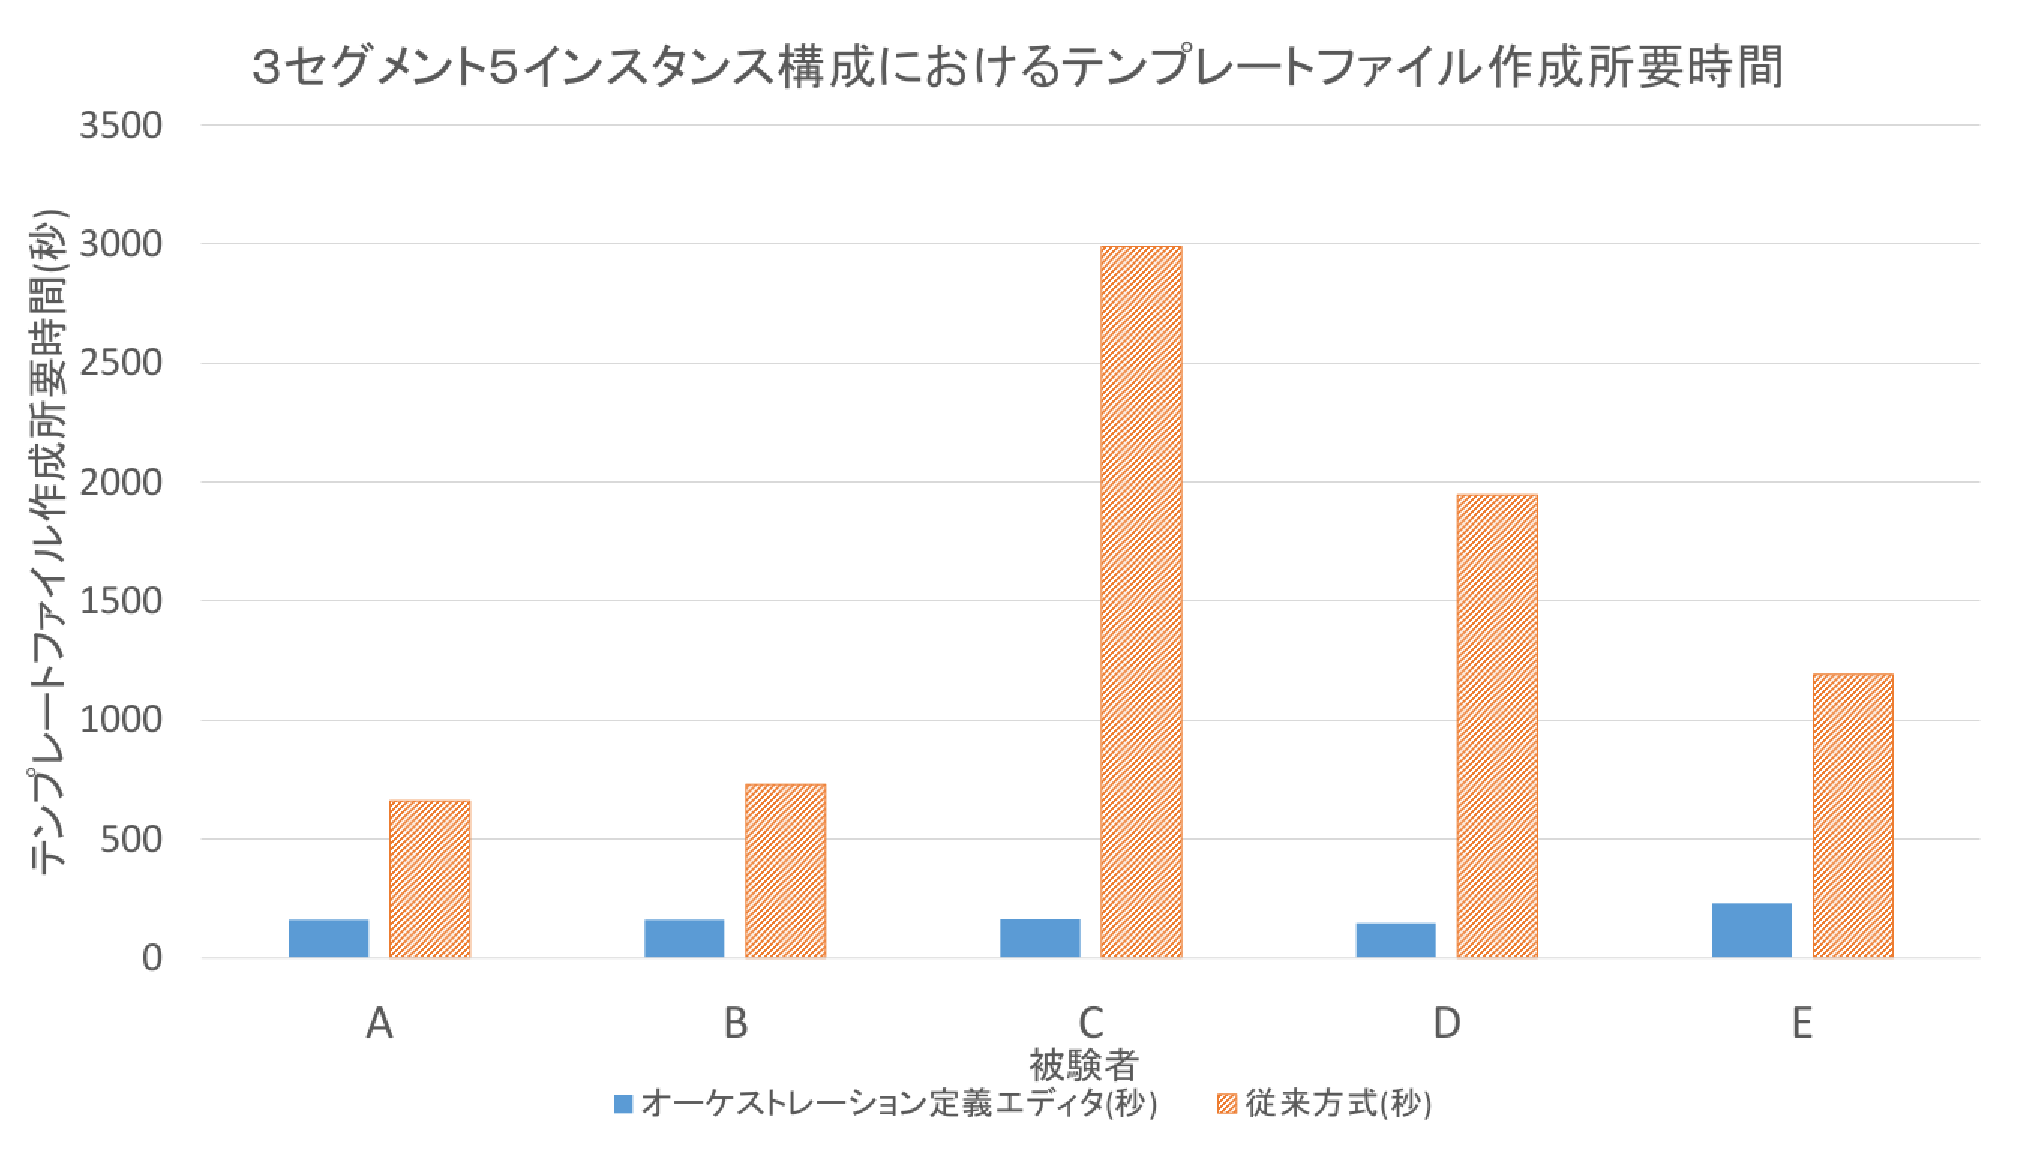
\includegraphics[scale=0.265]{Document/Abstract_Comparison.eps}
 		\caption{テンプレートファイル作成所要時間}
 		\label{graf:2}
 	\end{center}
 \end{figure}
 被験者全員が,全てのシステム構成構築において入力量を削減することができ,作成所要時間を大幅に短縮された.
% \begin{itemize} \vspace*{-1zh}
%  \item 適応度比例戦略による複製 \vspace*{-1zh}
%  \item OX,PMX,CX という 3 種類の交叉 \vspace*{-1zh}
%  \item ランダムに選ばれた 2 点の遺伝子を交換する突然変異 \vspace*{-1zh}
%  \item 2-opt アルゴリズムによる部品挿入順序の局所最適化 \vspace*{-1zh}
% \end{itemize}
% という流れを繰り返す.
 
 \section{まとめ}
 本研究ではOpenStack内コンポーネントであるHeatを用いたオーケストレーション時に問題となっていた入力量の多さと構築内容の把握しづらさを解決するためにオーケストレーション定義エディタを実装.これにより従来方式に比べてテンプレートファイル作成所要時間を大幅短縮,構築内容もGUIにて可視化されHeatテンプレートファイルをより容易に作成可能にした.
% \vspace{-2zh}
% \begin{table}[hbtp]
%  \begin{center}
%   \caption{実験結果}
%   \label{tab:result}
%   \begin{tabular}{|c|c||r|r|r|r|} \hline
%	\multicolumn{2}{|c||}{Data}	&
%	\multicolumn{2}{c|}{Prev.}	&
%	\multicolumn{2}{c|}{our method}	\\ \hline
%	部品数	& 品種数&
%	\multicolumn{1}{c|}{Best} & \multicolumn{1}{c|}{Time} &
%	\multicolumn{1}{c|}{Best} & \multicolumn{1}{c|}{Time}	\\ \hline\hline
%			& 10	& 10	&   250.0	&  2	&   48.5	\\ \cline{2-6}
%	\lw{100}& 20	& 30	&   336.2	& 16	&   70.5	\\ \cline{2-6}
%			& 30	& 50	&   347.1	& 40	&   98.7	\\ \cline{2-6}
%			& 40	& 66	&   363.3	& 58	&  168.4	\\ \hline
%			& 10	& 14	&  2346.3	&  0	&  196.8	\\ \cline{2-6}
%	\lw{200}& 20	& 36	&  2840.8	& 19	&  302.0	\\ \cline{2-6}
%	 		& 30	& 57	&  2770.0	& 38	&  578.9	\\ \cline{2-6}
%	 		& 40	& 87	&  3300.8	& 64	&  723.2	\\ \hline
%			& 10	&  6	&  8457.6	&  1	&  391.5	\\ \cline{2-6}
%	\lw{300}& 20	& 31	&  9938.1	& 12	&  724.7	\\ \cline{2-6}
%	 		& 30	& 58	& 11092.8	& 31	& 1309.5	\\ \cline{2-6}
%	 		& 40	& 89	& 12345.4	& 51	& 1577.2	\\ \hline
%   \end{tabular}
%  \end{center}
% \end{table}
% \vspace{-2zh}
 
%% 参考文献 %%%%%%%%%%%%%%%%%%%%%%%%%%%%%%%%%%%%%%%%%%%%%%%%%%%%%%%%%%%%
\begin{thebibliography}{99}
 \bibitem{Document:1} OpenStack,\url{https://www.openstack.org/}
\end{thebibliography}

\end{Abstract}
\end{document}
